\section{Entanglement generation}\label{sec:4:entanglement-generation}
If the full state $\rho$ is measured repeatedly but for each measurement the initial setup was slightly different, this effectively is an averaging process over all the variations in the setup.
As mentioned earlier, this averaging mixes the state and for large variations $\Delta \theta$ and $\Delta L$, this process can destroy entanglement.
To see this, we calculate the averaged state $\mean{\rho}$ as
\begin{equation}\label{eq:4:average-density}
  \mean{\rho} = \int_{\infty}^{\infty} \dd \theta_A p(\theta_A) \int_{\infty}^{\infty} \dd \theta_B p(\theta_B) \int_{\infty}^{\infty} \dd L_A p(L_A) \int_{\infty}^{\infty} \dd L_B p(L_B) \ \rho(\theta_A, \theta_B, L_A, L_B)
\end{equation} 
where $p(\,\cdot\,)$ is the gaussian probability distribution. For both, $\theta$ and $L$, this is distributed around mean $0$ and with standard deviation $\Delta \theta$ and $\Delta L$. $\rho(\theta_A, \theta_B, L_A, L_B)$ is the state of a single measurement, dependent on the parameters $\theta_i$ and $L_i$ of the setup.
This state is very similar as before in \cref{cha:first-look} but with the additional effect of the casimir interactions taken into account.
The initial state $\ket{\psi_0}$ at $t=0$ is given by eq. \eqref{eq:2:initial-state}.
During the time evolution, not only the mutual gravitational interactions between the masses but also the Casimir interactions between the shield and the states has to be taken into account. A state $\ket{\psi^i_{A(B)}}$ ($i = 1, 2$) accumulated the phase $\phi^i_{A(B),\,\mathrm{Cas}}(t)$ during time evolution.
This phase is given by
\begin{equation}
  \phi^i_{A(B),\,\mathrm{Cas}}(t) = \frac{t}{\hbar}
  \begin{cases}
     \frac{3 \hbar c}{8 \pi} \left(\frac{\varepsilon_r - 1}{\varepsilon_r + 2}\right) \frac{R^3}{(L^i_{A(B)})^4} & \text{for large separations (LSL)} \\
    \frac{\hbar c \pi^3}{720} \varphi(\varepsilon_r) \left(\frac{\varepsilon_r - 1}{\varepsilon_r + 1}\right) \frac{R}{(\mathscr{L}^i_{A(B)})^2} & \text{for small separations (PFA)}
  \end{cases}
\end{equation}
where a distinction between the different Casimir-models discussed in \cref{cha:casimir-effect} has been made.
The plate-sphere separations $L^i_{A(B)}$ and $\mathscr{L}^i_{A(B)} = L^i_{A(B)}-R$ are of course dependent on the placement of the particles.
In full generality, they are given by
\begin{equation}
  L^i_{A(B)} = L + L_{A(B)} - \frac{d}{2} \pm \frac{\Delta x_{A(B)}}{2} \sin(\xi + \theta_{A(B)})
\end{equation}
where $\pm$ depends on the considered state and $\xi = \alpha, \beta$ was used as an abbreviation.
The mutual gravitational interaction for states $\ket{\psi^i_A}\otimes\ket{\psi^j_B}$ is given similar to before by the accumulated phase
\begin{equation}
  \phi^{ij}_\mathrm{Grav}(t) = \frac{t}{\hbar} \frac{G M_A M_B}{L^{ij}} .
\end{equation}
The separation between the spheres $L^{ij}$ ($i,j = 1,2$) in full generality is given by
\begin{multline}
  L^{ij} = \sqrt{\left(2L + L_A + L_B \pm \frac{\Delta x_A}{2}\sin(\alpha + \theta_A) \mp \frac{\Delta x_B}{2}\sin(\beta + \theta_B)\right)^2 +} \\ \overline{\left(\frac{\Delta x_A}{2}\cos(\alpha + \theta_A) \pm \frac{\Delta x_B}{2}\cos(\beta + \theta_B)\right)^2}
\end{multline}
Expanding both phases in first order of $\Delta x_{A(B)}$ as already done before and in $\theta_{A(B)} \ll 1$, $L_{A(B)} \ll 1$ (which is feasible as both are very small as seen later), the averaging in eq. \eqref{eq:4:average-density} can be performed analytically (see \cref{apx:average-density}).
It turns out, that with $\Delta \theta_A = \Delta \theta_B \equiv \Delta\theta$ and $\Delta L_A = \Delta L_B \equiv \Delta L$ all off-diagonal elements of the averaged state $\mean{\rho}$ are given in the form
\begin{equation}\label{eq:4:average-density-element}
  \mean{\rho_{kl}} = \frac{1}{4} e^{i \Delta \phi_{kl}(t)} \exp{-\frac{(\Delta\theta)^2}{2} (\Delta\phi_{kl,\,\theta})^2 t^2} \exp{-\frac{(\Delta L)^2}{2} (\Delta\phi_{kl,\,L})^2 t^2}
\end{equation}
where all $\Delta \phi$-terms are replacements for rather lengthy linearized phase expressions which depend on the separation $L$, the orientation $\alpha, \beta$, the masses $M_{A(B)}$ and the delocalization size $\Delta x_{A(B)}$.
It becomes evident, that for large times or for large variations in the placement, these off-diagonal elements tend to zero. 
For $t\rightarrow \infty$ or for $\Delta \theta, \Delta L \rightarrow \infty$, this state represents the maximally mixed state with $\tr\rho^2 = 1/4$, which obviously is not entangled.
For large variations in the placement, one therefore expects a loss of entanglement.

The resulting logarithmic negativity of the averaged state $E_N(\mean{\rho})$ was computed numerically for different values of $\Delta \theta$ and $\Delta L$ and is shown in \cref{fig:4:EN-delta-theta}.
\begin{figure}[!htb]
  \centering
  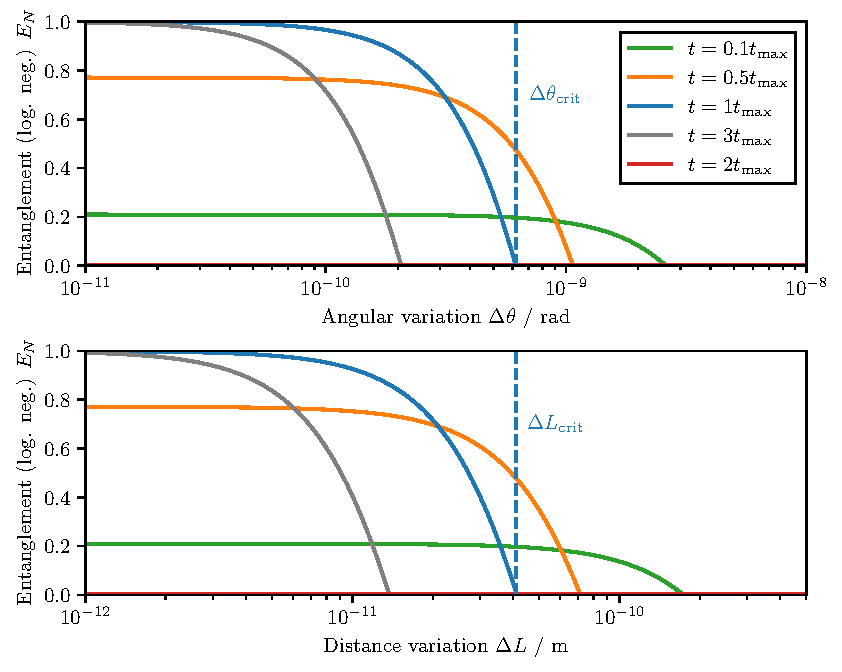
\includegraphics[width=\textwidth]{./../figures/theta-variance/EN-deltaTheta-deltaL.pdf}
  \caption{Entanglement quantified by the logarithmic negativity (eq. \eqref{eq:2:logarithmic-negativity}) dependent on the angular variation $\Delta\theta$ and the distance variation $\Delta L$ in the parallel configuration. The entanglement is shown at different times, where $t_\mathrm{max} \approx 258\si{ms}$ is the time of maximal entanglement from eq. \eqref{eq:2:t-max-parallel}. At a critical point $\Delta \theta_\mathrm{crit}$ and $\Delta L_\mathrm{crit}$ all entanglement is lost.}
  \label{fig:4:EN-delta-theta}
\end{figure}
For this figure, the parallel configuration with $\alpha = \beta = 0$ was used with $t_\mathrm{max}$ given by eq. \eqref{eq:2:t-max-parallel} as well as a radius $R=1\times 10^{-5}\si{m}$, a corresponding mass of $M_A = M_B = 4/3\, \pi R^3 \rho_\mathrm{Silica} \approx 1.1\times 10^{-11}\si{kg}$, a separation of $L=2R$ and a superposition size of $\Delta x_A = \Delta x_B = 100\si{nm}$.
In the rest of the thesis, if not otherwise specified, these parameters are used as a default.
They are chosen in these orders of magnitude, because they result in a feasible low experiment-time $t_\mathrm{max}\approx 258\si{ms}$ and are in the region of what is soon\footnote{\q{Soon} in this context means still a long time, but it could be reachable within the next century.} possible \cite{Aspelmeyer_2024}.
It is important however to stress out, that all these parameters are orders of magnitude away of from what is experimentally reachable today.
The largest mass that was studied in matter-wave interferometry is in the order of $4\times 10^{-23}\si{kg}$ \cite{Fein_2019} with an superposition size of $\Delta x > 500\si{nm}$.
For solid state mechanical systems quantum control up to masses of order $10^{-13}\si{kg}$ \cite{OConnell_2010}, $10^{-11}\si{kg}$ \cite{Lee_2011} and $10^{-11}\si{kg}$ \cite{Bild_2023} but with very short coherence times $\lesssim 1\si{\mu s}$ have been demonstrated.
On the contrary, the smallest mass with measured gravity is around $92 \si{mg}$ \cite{Westphal_2021}.
Levitated particles combine the best of both world with quantum control of large and heavy trapped solid objects as well as long coherence times up to the order of seconds \cite{Aspelmeyer_2024}.

The entanglement of the system shown in \cref{fig:4:EN-delta-theta} behaves as expected. At some critical point $\Delta \theta_\mathrm{crit}$ and $\Delta L_\mathrm{crit}$, the entanglement is completely lost.
For the used parameters and in the parallel orientation, this threshold is around $\Delta \theta_\mathrm{crit} \approx 6 \times 10^{-10} \si{rad}$ and $\Delta L_\mathrm{crit} \approx 1.4 \times 10^{-10} \si{m}$, which seems quite challenging experimentally.
However, it seems like that for smaller times $t<t_\mathrm{max}$ larger variations can be tolerated for the cost of having less total entanglement.
This again is expected. For smaller times, the gravitational force did not have enough time to fully entangle the two particles, but also the decoherences (dependent on $\propto t^2$ in eq. \eqref{eq:4:average-density-element}) did not have enough time to built up. 
It is therefore logical, that if one does not require to measure a fully entangled state and less entanglement $E_N < 1$ is also sufficient, it may be beneficial to measure at a time $t < t_\mathrm{max}$. 
This does not only reduce the time of a single experimental run, but also increases the stability against displacement variations. This optimal time of measuring for a certain required amount of entanglement is shown in \cref{fig:4:time-delta-theta}.
\begin{figure}[!htb]
  \centering
  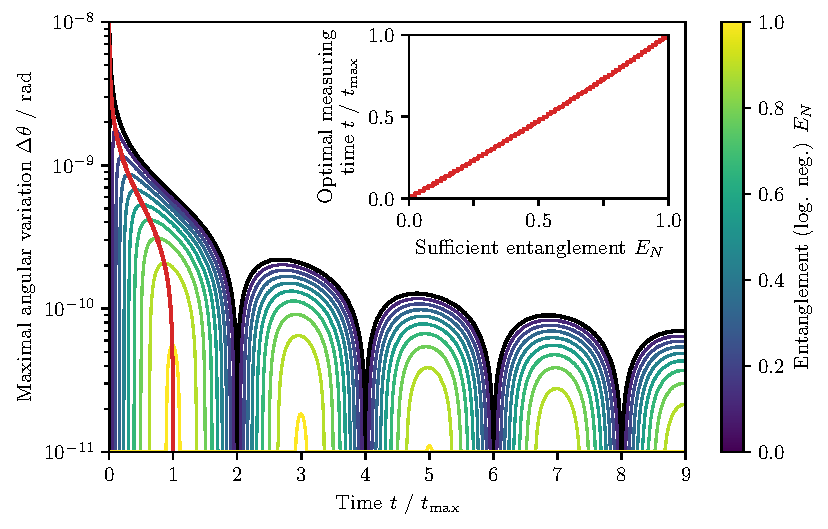
\includegraphics[width=\textwidth]{./../figures/theta-variance/time-delta-theta-crit-EN.pdf}
  \caption{Maximal angular variation for a given time and a given required amount of entanglement. The outer most black line corresponds to the time dependence of $\Delta \theta_\mathrm{crit}$. The top left as well as the red curve in the main figure shows the optimal measuring time for a sufficient amount of entanglement.
  At times $2k t_\mathrm{max}$ no entanglement can be measured.}
  \label{fig:4:time-delta-theta}
\end{figure}
The chart lets one read out the optimal measuring time $t$ for a sufficient amount of entanglement as well as the corresponding maximal angular variation for this to be possible.
On the other hand, if one is experimentally limited by a certain maximal angular variation, the corresponding best measuring time as well as the amount of entanglement one maximally gets can be read out.
It becomes evident, that at times $2k t_\mathrm{max}$, $k\in\mathbb{N}$ there is no entanglement present.
This aligns with the findings form the ideal scenario in \cref{cha:first-look}. 